% Options for packages loaded elsewhere
\PassOptionsToPackage{unicode}{hyperref}
\PassOptionsToPackage{hyphens}{url}
%
\documentclass[
  english,
  man, donotrepeattitle,floatsintext]{apa7}
\title{Data irregularities across six implicit learning articles: Comments on Lola, Giatis, Pérez-Turpin, and Tzetzis (2021), Lola and Tzetzis (2021), Lola and Tzetzis (2020), Tzetzis and Lola (2015), Lola, Tzetzis, and Zetou (2012), and Tzetzis and Lola (2010)}
\author{Brad McKay\textsuperscript{1} \& Michael J. Carter\textsuperscript{1}}
\date{}

\usepackage{amsmath,amssymb}
\usepackage{lmodern}
\usepackage{iftex}
\ifPDFTeX
  \usepackage[T1]{fontenc}
  \usepackage[utf8]{inputenc}
  \usepackage{textcomp} % provide euro and other symbols
\else % if luatex or xetex
  \usepackage{unicode-math}
  \defaultfontfeatures{Scale=MatchLowercase}
  \defaultfontfeatures[\rmfamily]{Ligatures=TeX,Scale=1}
\fi
% Use upquote if available, for straight quotes in verbatim environments
\IfFileExists{upquote.sty}{\usepackage{upquote}}{}
\IfFileExists{microtype.sty}{% use microtype if available
  \usepackage[]{microtype}
  \UseMicrotypeSet[protrusion]{basicmath} % disable protrusion for tt fonts
}{}
\makeatletter
\@ifundefined{KOMAClassName}{% if non-KOMA class
  \IfFileExists{parskip.sty}{%
    \usepackage{parskip}
  }{% else
    \setlength{\parindent}{0pt}
    \setlength{\parskip}{6pt plus 2pt minus 1pt}}
}{% if KOMA class
  \KOMAoptions{parskip=half}}
\makeatother
\usepackage{xcolor}
\IfFileExists{xurl.sty}{\usepackage{xurl}}{} % add URL line breaks if available
\IfFileExists{bookmark.sty}{\usepackage{bookmark}}{\usepackage{hyperref}}
\hypersetup{
  pdftitle={Data irregularities across six implicit learning articles: Comments on Lola, Giatis, Pérez-Turpin, and Tzetzis (2021), Lola and Tzetzis (2021), Lola and Tzetzis (2020), Tzetzis and Lola (2015), Lola, Tzetzis, and Zetou (2012), and Tzetzis and Lola (2010)},
  pdfauthor={Brad McKay1 \& Michael J. Carter1},
  pdflang={en-EN},
  pdfkeywords={Metascience; GRIMMER; Effect sizes; Perceptual motor learning},
  hidelinks,
  pdfcreator={LaTeX via pandoc}}
\urlstyle{same} % disable monospaced font for URLs
\usepackage{graphicx}
\makeatletter
\def\maxwidth{\ifdim\Gin@nat@width>\linewidth\linewidth\else\Gin@nat@width\fi}
\def\maxheight{\ifdim\Gin@nat@height>\textheight\textheight\else\Gin@nat@height\fi}
\makeatother
% Scale images if necessary, so that they will not overflow the page
% margins by default, and it is still possible to overwrite the defaults
% using explicit options in \includegraphics[width, height, ...]{}
\setkeys{Gin}{width=\maxwidth,height=\maxheight,keepaspectratio}
% Set default figure placement to htbp
\makeatletter
\def\fps@figure{htbp}
\makeatother
\setlength{\emergencystretch}{3em} % prevent overfull lines
\providecommand{\tightlist}{%
  \setlength{\itemsep}{0pt}\setlength{\parskip}{0pt}}
\setcounter{secnumdepth}{-\maxdimen} % remove section numbering
% Make \paragraph and \subparagraph free-standing
\ifx\paragraph\undefined\else
  \let\oldparagraph\paragraph
  \renewcommand{\paragraph}[1]{\oldparagraph{#1}\mbox{}}
\fi
\ifx\subparagraph\undefined\else
  \let\oldsubparagraph\subparagraph
  \renewcommand{\subparagraph}[1]{\oldsubparagraph{#1}\mbox{}}
\fi
\newlength{\cslhangindent}
\setlength{\cslhangindent}{1.5em}
\newlength{\csllabelwidth}
\setlength{\csllabelwidth}{3em}
\newlength{\cslentryspacingunit} % times entry-spacing
\setlength{\cslentryspacingunit}{\parskip}
\newenvironment{CSLReferences}[2] % #1 hanging-ident, #2 entry spacing
 {% don't indent paragraphs
  \setlength{\parindent}{0pt}
  % turn on hanging indent if param 1 is 1
  \ifodd #1
  \let\oldpar\par
  \def\par{\hangindent=\cslhangindent\oldpar}
  \fi
  % set entry spacing
  \setlength{\parskip}{#2\cslentryspacingunit}
 }%
 {}
\usepackage{calc}
\newcommand{\CSLBlock}[1]{#1\hfill\break}
\newcommand{\CSLLeftMargin}[1]{\parbox[t]{\csllabelwidth}{#1}}
\newcommand{\CSLRightInline}[1]{\parbox[t]{\linewidth - \csllabelwidth}{#1}\break}
\newcommand{\CSLIndent}[1]{\hspace{\cslhangindent}#1}
% Manuscript styling
\usepackage{upgreek}
\captionsetup{font=singlespacing,justification=justified}

% Table formatting
\usepackage{longtable}
\usepackage{lscape}
% \usepackage[counterclockwise]{rotating}   % Landscape page setup for large tables
\usepackage{multirow}		% Table styling
\usepackage{tabularx}		% Control Column width
\usepackage[flushleft]{threeparttable}	% Allows for three part tables with a specified notes section
\usepackage{threeparttablex}            % Lets threeparttable work with longtable

% Create new environments so endfloat can handle them
% \newenvironment{ltable}
%   {\begin{landscape}\begin{center}\begin{threeparttable}}
%   {\end{threeparttable}\end{center}\end{landscape}}
\newenvironment{lltable}{\begin{landscape}\begin{center}\begin{ThreePartTable}}{\end{ThreePartTable}\end{center}\end{landscape}}

% Enables adjusting longtable caption width to table width
% Solution found at http://golatex.de/longtable-mit-caption-so-breit-wie-die-tabelle-t15767.html
\makeatletter
\newcommand\LastLTentrywidth{1em}
\newlength\longtablewidth
\setlength{\longtablewidth}{1in}
\newcommand{\getlongtablewidth}{\begingroup \ifcsname LT@\roman{LT@tables}\endcsname \global\longtablewidth=0pt \renewcommand{\LT@entry}[2]{\global\advance\longtablewidth by ##2\relax\gdef\LastLTentrywidth{##2}}\@nameuse{LT@\roman{LT@tables}} \fi \endgroup}

% \setlength{\parindent}{0.5in}
% \setlength{\parskip}{0pt plus 0pt minus 0pt}

% Overwrite redefinition of paragraph and subparagraph by the default LaTeX template
% See https://github.com/crsh/papaja/issues/292
\makeatletter
\renewcommand{\paragraph}{\@startsection{paragraph}{4}{\parindent}%
  {0\baselineskip \@plus 0.2ex \@minus 0.2ex}%
  {-1em}%
  {\normalfont\normalsize\bfseries\itshape\typesectitle}}

\renewcommand{\subparagraph}[1]{\@startsection{subparagraph}{5}{1em}%
  {0\baselineskip \@plus 0.2ex \@minus 0.2ex}%
  {-\z@\relax}%
  {\normalfont\normalsize\itshape\hspace{\parindent}{#1}\textit{\addperi}}{\relax}}
\makeatother

% \usepackage{etoolbox}
\makeatletter
\patchcmd{\HyOrg@maketitle}
  {\section{\normalfont\normalsize\abstractname}}
  {\section*{\normalfont\normalsize\abstractname}}
  {}{\typeout{Failed to patch abstract.}}
\patchcmd{\HyOrg@maketitle}
  {\section{\protect\normalfont{\@title}}}
  {\section*{\protect\normalfont{\@title}}}
  {}{\typeout{Failed to patch title.}}
\makeatother

\usepackage{xpatch}
\makeatletter
\xapptocmd\appendix
  {\xapptocmd\section
    {\addcontentsline{toc}{section}{\appendixname\ifoneappendix\else~\theappendix\fi\\: #1}}
    {}{\InnerPatchFailed}%
  }
{}{\PatchFailed}
\keywords{Metascience; GRIMMER; Effect sizes; Perceptual motor learning}
\usepackage{lineno}

\linenumbers
\usepackage{csquotes}
\usepackage{pdflscape}
\usepackage{xcolor}
\raggedbottom
\pagewiselinenumbers
\ifXeTeX
  % Load polyglossia as late as possible: uses bidi with RTL langages (e.g. Hebrew, Arabic)
  \usepackage{polyglossia}
  \setmainlanguage[]{english}
\else
  \usepackage[main=english]{babel}
% get rid of language-specific shorthands (see #6817):
\let\LanguageShortHands\languageshorthands
\def\languageshorthands#1{}
\fi
\ifLuaTeX
  \usepackage{selnolig}  % disable illegal ligatures
\fi


\shorttitle{Commentary on Lola \& Tzetzis papers}

\authornote{

\vspace{-.5cm} 
\addORCIDlink{Brad McKay}{0000-0002-7408-2323}
\newline \indent \addORCIDlink{Michael J. Carter}{0000-0002-0675-4271}

Correspondence concerning this article should be addressed to Brad McKay, 1280 Main Street West, Ivor Wynne Centre Room AB-131 A1, McMaster University, Hamilton ON Canada, L8S 4K1. E-mail: \href{mailto:bradmckay8@gmail.com}{\nolinkurl{bradmckay8@gmail.com}}

}

\affiliation{\vspace{0.5cm}\textsuperscript{1} Department of Kinesiology, McMaster University}

\note{

\vspace{\baselineskip}

\raggedright Submitted to \emph{Meta-Psychology}. Participate in open peer review by commenting through hypothes.is directly on this preprint. The full editorial process of all articles under review at \emph{Meta-Psychology} can be found here: \url{https://tinyurl.com/mp-submissions}. You will find this preprint by searching for the first author's name.

}

\abstract{
We present a critical re-analysis of six implicit learning papers published by the same authors between 2010 and 2021. We calculated effect sizes for each pairwise comparison reported in the papers using the data published in each article. We further identified mathematically impossible data reported in multiple papers, either with deductive logic or by conducting a GRIMMER analysis of reported means and standard deviations. We found the pairwise effect sizes were implausible in all six articles in question, with Cohen's \emph{d} values often exceeding 100 and sometimes exceeding 1000. \textcolor{red}{In contrast, the largest effect size observed in a million simulated experiments with a true effect of $d$ = 3 was $d$ = 6.6.} Impossible statistics were reported in four out of the six articles. Reported test statistics and \(\eta^{2}\) values were also implausible, with several \(\eta^{2}\) = .99 and even \(\eta^{2}\) = 1.0 for between-subjects main effects. The results reported in the six articles in question are unreliable. Many of the problems we identified could be spotted without further analysis, highlighting the need for adequate statistical training in the field of motor learning.
}



\begin{document}
\maketitle

Statistical reporting errors may commonly occur in psychology articles (Brown \& Heathers, 2017; Nuijten, Hartgerink, van Assen, Epskamp, \& Wicherts, 2016) and such errors are often consistent with hypothesized results (Bakker \& Wicherts, 2011). When the primary conclusions in research articles depend on reporting errors, replicability is unlikely and future research may be wasted if researchers attempt to build on the erroneously reported results (Munafò et al., 2017). In this paper, we scrutinize six papers published by the same two authors\footnote{One of the six papers had a third author and one had a third and fourth author.}, where the authors report a high number of erroneous or implausible data on which their primary conclusions depend. We first became aware of the Lola and Tzetzis (2021) paper when the paper was highlighted in a social media post (Gray, 2021). During an initial read through by one of us (BM), a number of reporting and statistical issues were noticed. The paper also referenced past research published by these authors. Given our concerns over the issues found in the Lola and Tzetzis (2021) paper, we deemed it necessary to examine these other papers. We remain agnostic to the sources of error in each of these papers. Nevertheless, the data irregularities we found are similar across the target articles and at times even include repeated values (e.g., \(F\)-statistics) across multiple papers. Regardless of the conclusion one reaches with respect to the mechanism behind these errors, it is our contention that the results reported in these papers are unreliable and that the respective journals in which the papers are published should take corrective actions\footnote{On Sept 22 2021, we contacted the journal editors \textcolor{red}{of all articles except} Lola et al. (2021) \textcolor{red}{as we were unaware of this article at the time}. The Editors indicated their intention to further investigate these issues and/or take corrective actions. \textcolor{red}{On Jan 21 2022, we contacted the journal editor regarding the} Lola et al. (2021) \textcolor{red}{article.}}. Below, we outline our causes for concern and the overarching issues we found across the six articles in question.

\hypertarget{the-articles-in-question}{%
\subsection{The Articles in Question}\label{the-articles-in-question}}

\textcolor{red}{We reanalyzed the following six articles by Afroditi Lola and George Tzetzis:}

\begin{enumerate}
\def\labelenumi{\arabic{enumi}.}
\item
  Lola, A.C., Giatsis, G., Pérez-Turpin, J.A., \& Tzetzis, G.C. (2021). The influence of analogies on the development of selective attention in novices in normal or stressful conditions. \emph{Journal of Human Sport and Exercise}. \url{https://doi.org/10.14198/jhse.2023.181.12}
\item
  Lola, A.C., \& Tzetzis, G.C. (2021). The effect of explicit, implicit and analogy instruction on decision making skill for novices, under stress. \emph{International Journal of Sport and Exercise Psychology}, 1-21. \url{https://doi.org/10.1080/1612197X.2021.1877325}
\item
  Lola, A.C., \& Tzetzis, G.C. (2020). Analogy versus explicit and implicit learning of a volleyball skill for novices: The effect on motor performance and self-efficacy. \emph{Journal of Physical Education and Sport}, 20(5), 2478-2486. \url{https://doi.org/10.7752/jpes.2020.05339}
\item
  Tzetzis, G.C., \& Lola, A.C. (2015). The effect of analogy, implicit, and explicit learning on anticipation in volleyball serving. \emph{International Journal of Sport Psychology}, 46(2), 152-166. \url{https://doi.org/10.7352/IJSP.2015.46.152}
\item
  Lola, A.C., \& Tzetzis, G.C., \& Zetou, H. (2012). The effect of implicit and explicit practice in the development of decision making in volleyball serving. \emph{Perceptual and Motor Skills}, 114(2), 665-678. \url{https://doi.org/10.2466/05.23.25.PMS.114.2.665-678}
\item
  Tzetzis, G.C., \& Lola, C.A. (2010). The role of implicit, explicit instruction and their combination in learning anticipation skill, under normal and stress conditions. \emph{International Journal of Sport Sciences and Physical Education}, 1, 54-59.\footnote{This journal has been identified as a potential predatory journal. We were unable to find an online version of this article on the journal's webpage and interestingly, the earliest issue on the webpage is from 2016. We were only able to find an online version on ResearchGate (\url{https://www.researchgate.net/profile/Angela-Calder/publication/234000504_The_scientific_basis_for_recovery_training_practices_in_sport/links/5428fff80cf26120b7b574ad/The-scientific-basis-for-recovery-training-practices-in-sport.pdf\#page=57}).}
\end{enumerate}

\textcolor{red}{In all experiments, the authors investigated the effects of implicit and explicit instructions on perceptual and motor learning. All experiments sampled young females who were enrolled in a volleyball camp} (see Table \ref{tab:table1}). \textcolor{red}{Our reanalysis of the target articles evaluated the plausibility of the reported means, standard deviations, and test statistics.}

\vspace{3ex}

\begin{table}

\caption{\label{tab:table1}Participant demographics in each of the target articles.}
\fontsize{11}{13}\selectfont
\begin{threeparttable}
\begin{tabular}[t]{ll}
\toprule
Target article & Sample size and participant details\\
\midrule
Lola et al (2021) & 60 females, age range: 11 to 12 years ($M_{age}$ and SD not reported)\\
Lola \& Tzetzis (2021) & 60 females, age range: 10 to 11 years ($M_{age}$ = 10.48, SD = 0.911)\textsuperscript{a}\\
Lola \& Tzetzis (2020) & 80 females, age range: 10 to 11 years ($M_{age}$ = 10.48, SD = 0.911)\textsuperscript{a}\\
Tzetzis \& Lola (2015) & 60 females, age range: 9 to 12 years ($M_{age}$ = 10.48, SD = 0.91)\textsuperscript{a}\\
Lola et al (2012) & 60 females, age range: 10 to 12 years ($M_{age}$ = 11.2, SD = 0.3)\\
Tzetzis \& Lola (2010) & 48 females, age range: 12 to 13 years ($M_{age}$ = 12.38, SD = 0.34)\\
\bottomrule
\end{tabular}
\begin{tablenotes}
\item \textit{Note.} 
\item[a] These articles report identical means and standard deviations for the age of their participants despite a different sample size in Lola \& Tzetzis 2020 from Lola \& Tzetzis 2021 and Tzetzis \& Lola 2015, and a different age range in Tzetzis \& Lola 2015 from Lola \& Tzetzis 2020 and 2021
\end{tablenotes}
\end{threeparttable}
\end{table}

Although there were some differences between the reported experiments in the target articles, there were many methodological commonalities that can be summarized. All six articles involved female children learning a volleyball skill as part of a volleyball camp. In each case, the participants were reported to have minimal experience (i.e., were described as novices) with the task at hand. The purpose of all six experiments was to evaluate perceptual or motor learning differences as a function of the type of instruction received during practice. Each experiment included a pre-test, an acquisition (i.e., practice) phase involving 12 sessions spaced over four weeks, and a post-test. A high stress test was also included in Lola et al. (2021), Lola and Tzetzis (2021), and Tzetzis and Lola (2010).

In Lola et al. (2021), Lola and Tzetzis (2021), Lola and Tzetzis (2020), and Tzetzis and Lola (2015), the groups differed with respect to the type of instruction received: implicit, explicit, or analogy. In Lola et al. (2012) and Tzetzis and Lola (2010), a sequential group (see below for description) replaced the analogy group. All six experiments also included a control group that did not practice the task. Implicit instruction did not contain any explicit information for how to perform the task and the learners were asked to perform a distracting task like counting backwards while practicing to prevent them from acquiring declarative rules for performance. In contrast, explicit instruction consisted of direct verbal instructions for performing the task. Analogy instruction was considered a type of implicit instruction wherein an analogy or metaphor was provided to the learner. For example, ``Imagine that the opponents' surface is covered with water. Send the ball where there is more water and no opponents at the court.'' (Lola \& Tzetzis, 2021, p. 9). Sequential instruction involved receiving explicit instruction for the first half of training followed by implicit instruction for the second half of training. Across experiments, the authors predicted that implicit forms of instruction---implicit, analogy, and sequential---would be more effective than explicit instruction for motor and perceptual learning. This advantage was also predicted to be greater when testing was conducted in a high stress situation. In Lola and Tzetzis (2021) for instance, high stress was induced by falsely telling participants that the best performers would be selected for a draft to the national team. Further, it was predicted that analogy or sequential instruction would offer improvements relative to implicit instruction.

The primary outcome measures used in these experiments were reaction time (Lola et al., 2021; Lola \& Tzetzis, 2021; Lola et al., 2012; Tzetzis \& Lola, 2010, 2015), response accuracy (Lola et al., 2021; Lola \& Tzetzis, 2021; Lola et al., 2012; Tzetzis \& Lola, 2015), and motor performance measured on a 4-point scale (Lola \& Tzetzis, 2020). In addition, Lola and Tzetzis (2021) and Tzetzis and Lola (2010) included a measure of state anxiety, the Competitive State Anxiety Inventory-2 (Tsorbatzoudis, Barkoukis, Kaissidis-Rodafinos, \& Grouios, 1998), and Lola and Tzetzis (2020) had a measure of self-efficacy using a Likert scale. The number of explicit rules recalled was assessed in Lola and Tzetzis (2021), Tzetzis and Lola (2015), Lola et al. (2012), and Tzetzis and Lola (2010).

\hypertarget{methods}{%
\section{Methods}\label{methods}}

None of the six articles in question included a link to a public repository where the data could be accessed. We first wrote (email sent February 10, 2021) the corresponding author of the Lola and Tzetzis (2021) paper and asked if they would be willing to share the data for this experiment. The authors' response was that the data could not be shared as they were not finished with their analyses and were in the process of running different tests (A. Lola, personal communication, February 12 2021). We followed up this email (sent February 12 2021) by asking whether they would instead be willing to share the data from their other articles (i.e., Lola \& Tzetzis, 2020; Lola et al., 2012; Tzetzis \& Lola, 2010, 2015) as these were less recent, and presumably all planned analyses had been completed. After a 2 week period with no response, we followed up with a third email (sent February 26 2021) and reiterated our interest in obtaining their data from any of these articles. The authors' response was that they were unable to share data from any of these articles because in some cases they no longer had the data and in other cases they had plans to conduct further analyses (A. Lola, personal communication, March 2 2021).

Our first two requests did not include any indication about our concerns regarding the data irregularities. Subsequently, in a fourth email (sent April 12 2021) we outlined our concerns for each article\footnote{Excluding Lola et al. (2021) article as it had not yet been accepted for publication.} and once again reiterated our request to the authors to share any available data for any of the target articles. These requests were once again refused. The authors did address some specific concerns regarding Lola and Tzetzis (2021), but for the most part only provided more general responses to our concerns. The authors admitted that some of the values reported in the other target articles were incorrect, but did not identify which values or articles. Despite this, the authors maintained that the data irregularities---identified in our email and described in this paper---do not impact the veracity of their analyses or conclusions (A. Lola, personal communication, April 22 2021). We illustrate below that the data \emph{and} analyses reported in each of the articles reviewed are unreliable. Our extracted data and analysis scripts can be accessed at the following link: \url{https://osf.io/raz6q/}.

\hypertarget{effect-size-calculations-and-simulations}{%
\subsection{Effect Size Calculations and Simulations}\label{effect-size-calculations-and-simulations}}

Means and standard deviations were extracted from each article for all measures and time points that were reported. Cohen's \emph{d} was calculated for each pairwise comparison using the \texttt{compute.es} package in \texttt{R}. To provide context, we simulated data from two groups of \emph{n} = 20, consistent with group sizes in Lola and Tzetzis (2020), which had the largest groups among the target articles. We ran simulations with true effect sizes of \emph{d} = .8 and \emph{d} = 3 one million times each and report the range of effect sizes observed in those simulations.

\hypertarget{mathematically-impossible-data-and-granularity-analysis}{%
\subsection{Mathematically Impossible Data and Granularity Analysis}\label{mathematically-impossible-data-and-granularity-analysis}}

In two of the articles in question, it was clear that some of the reported results were not mathematically possible based on the scale of measurement that was used. When outcomes were single item integers (a granularity of 1), such as the number of explicit rules recalled, we used a web application (\url{http://www.prepubmed.org/grimmer_sd/}) to conduct a granularity analysis (GRIMMER) of reported means and standard deviations (Anaya, 2016). GRIMMER builds off the original Granularity-Related Inconsistency of Means (GRIM) analysis (Brown \& Heathers, 2017), which leveraged the fact that the means of granular data are also granular. Given a data set of size \emph{N} and granularity \emph{G}, only means of granularity \(G/N\) are possible. Thus, all possible means for data of a given \emph{G} and \emph{N} can be enumerated, and only means that match these possibilities are considered GRIM-consistent. The GRIMMER analysis extends this test by also evaluating whether mean-standard deviation pairs are possible. First, the GRIM analysis is conducted to determine if the mean is GRIM-consistent. Next, lower and upper bounds of the standard deviation are calculated based on how many decimals (\emph{D}) are reported \((SD\pm[\frac{0.5}{10^{D}}])^{2}\). Then all possible variances between these bounds are enumerated, converted back to standard deviations, and rounded to the nearest \emph{D} decimals. The reported standard deviation is checked for a match with any of these values. Finally, the mean-variance pair is compared to possible mean-variance pairings (the GRIMMER test handles sample sizes between 5 and 99). Using GRIMMER, it is possible to determine if specific mean and standard deviation pairs are possible for data of a given sample size. To be conservative, we specified that we did not know whether the standard deviation was calculated for the sample or population, nor whether ambiguous values were rounded up or down. Mean and standard deviation pairs that are mathematically possible are considered GRIMMER consistent, while mean and standard deviation pairs that are not mathematically possible are GRIMMER inconsistent.

\hypertarget{eta-squared-eta2}{%
\subsection{\texorpdfstring{Eta-squared (\(\eta^{2}\))}{Eta-squared (\textbackslash eta\^{}\{2\})}}\label{eta-squared-eta2}}

Each of the articles reported only omnibus test statistics and then reported post-hoc analyses with symbols demarcating significant and non-significant differences. In response to our expression of concern, the authors suggested that many of the issues were due to misprints in the articles. Specifically, they indicated that the reported means and standard deviations in their tables were incorrect and the root of the errors had to be from them outsourcing the formatting of their tables. The authors then insisted that despite these typographic errors, their discussion of the results and corresponding conclusions were still accurate (A. Lola, personal communication, April 22, 2021). However, the test statistics reported for many analyses were implausibly large and the authors often reported \(\eta^{2}\) values associated with the omnibus test. Our examination of the reported \(\eta^{2}\) values revealed that, as with the reported pairwise comparisons, many were implausibly large.

\hypertarget{results}{%
\section{Results}\label{results}}

\hypertarget{implausible-effect-sizes}{%
\subsection{Implausible Effect Sizes}\label{implausible-effect-sizes}}

Cohen's \emph{d} is used to describe the standardized mean difference of an effect and values can range between 0 and infinity \textcolor{red}{in both the negative and positive direction. We calculated absolute values so that all effects were positive}. Cohen's \(d_{s}\) (Cohen, 1988) is the observed difference between group means divided by their pooled standard deviation (see Lakens, 2013 for a detailed discussion). Conventional benchmarks for small, medium, and large effects are \emph{d} = .2, .5, and .8, respectively (Cohen, 1962); however, this \emph{cargo-cult} approach to effect size interpretation has been heavily discouraged (see Correll, Mellinger, McClelland, \& Judd, 2020; Field, 2016; Lakens, 2013; Thompson, 2007 for discussions). Recently, an analysis of 6447 Cohen's \emph{d} statistics extracted from social psychology meta-analyses observed median and 75th percentile Cohen's \emph{d} values of .36 and .65, respectively---suggesting the conventional benchmarks may overestimate typical effects (Lovakov \& Agadullina, 2021). \textcolor{red}{In the field of motor learning, recent meta-analyses have found average effect sizes in the published literature of} \emph{d} = .19 (McKay et al., 2021), \emph{d} = .54 (McKay, Yantha, Hussien, Carter, \& Ste-Marie, in press), and \emph{d} = .71 (Lohse, Buchanan, \& Miller, 2016).

To evaluate the maximum plausible Cohen's \emph{d} statistics one might encounter from experiments similar to those reported in the target articles, we conducted two simulations that each consisted of one million experiments (see Figure \ref{fig:fig1}). We set the true effect size at \emph{d} = .8, the conventional benchmark for a ``large'' treatment effect, in the first simulation. The largest effect size observed from the one million simulated experiments was \emph{d} = 2.97. In the second simulation, we set the true effect size at \emph{d} = 3, an unrealistically large effect size that might rarely be encountered in the psychology and/or motor learning literature. The maximum effect size observed in the one million simulated experiments was \emph{d} = 6.6.



\begin{figure}

{\centering 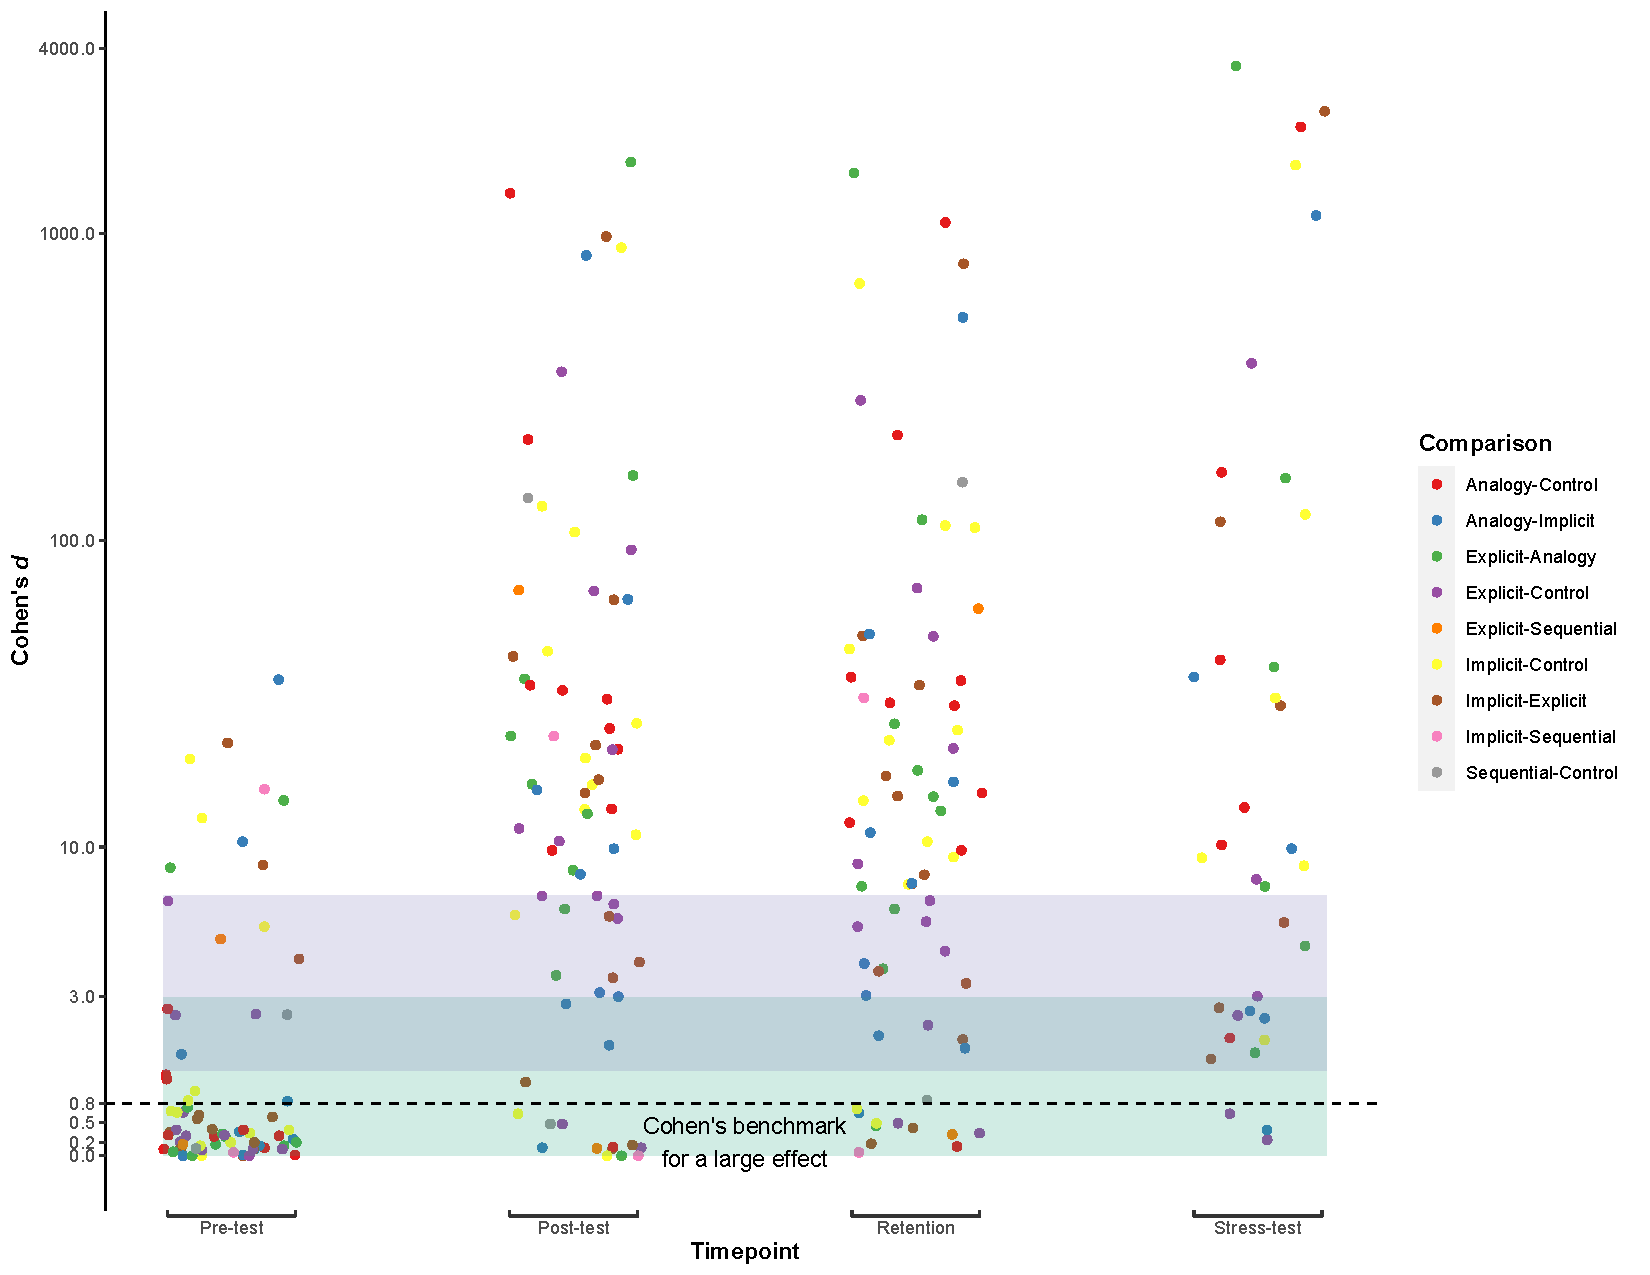
\includegraphics[width=1\linewidth,height=1\textheight]{../../figs/fig1b} 

}

\caption{Absolute Cohen's \(d\) estimates from all articles except Tzetzis and Lola (2010) plotted on a logarithmic scale. Only data from the original tables in Lola et al. (2021) are included. All pairwise comparisons have been included for all dependent measures in each experiment. The range of observed values from a simulation of 1,000,000 experiments with a true effect of \(d\) = .8 is illustrated by shaded green and blue regions of the figure, reaching a maximum value of \(d\) = 2.97. The range of observed values from a simulation of 1,000,000 experiments with a true effect of \(d\) = 3 is illustrated by the shaded purple and blue regions of the figure, reaching a maximum value of \(d\) = 6.6.}\label{fig:fig1}
\end{figure}

In the context of the maximum values observed in our simulations, all six articles in question reported implausibly large effect sizes. \textcolor{red}{The original table of summary statistics in} Lola et al. (2021) \textcolor{red}{indicated that} the smallest post-intervention difference in reaction times was \emph{d} = .64. However, all other effects were larger than \emph{d} = 8.7 and the largest effect was \emph{d} = 41. The accuracy data also reflected improbably large post-intervention differences, with two-thirds of all comparisons showing effects larger than \emph{d} = 5 and a largest effect of \emph{d} = 13.35. \textcolor{red}{However, a correction to the tables of summary statistics was published that included substantially smaller standard deviations than the original tables. While the updated data do imply smaller effect sizes, as we discuss below, they appear to be inconsistent with the reported analyses.}

In Lola and Tzetzis (2021), the smallest pre-test difference for reaction time was \emph{d} = 1.29 and the largest pre-test difference was \emph{d} = 35.32---although none of the groups were reported as significantly different in the article. The smallest post-intervention effect at any of the three time points was \emph{d} = 286.42, while the largest effect was \emph{d} = 3504.86. A similar picture emerges when analyzing the accuracy data. All the pre-test differences were improbably large (all \emph{d}'s \(\geq\) 2.52) despite being reported as not significantly different in the articles. Ten of the pairwise comparisons resulted in \emph{d}'s \(\geq\) 100 following treatment with the independent variables. The motor component data revealed post-treatment effect sizes ranging from \emph{d} = 1.16 to \emph{d} = 13.5.

In Lola and Tzetzis (2020), post-intervention motor performance effect sizes ranged from \emph{d} = 3.1 to \emph{d} = 20.95. Similarly, post-intervention self-efficacy effect sizes ranged from \emph{d} = 1.79 to \emph{d} = 44.46. Likewise, in Tzetzis and Lola (2015) post-intervention reaction time effect sizes ranged from \emph{d} = 2.28 to \emph{d} = 35.97. Continuing this pattern, post-intervention response accuracy effect sizes ranged from \emph{d} = 5.84 to \emph{d} = 29.7.

In Lola et al. (2012), many response accuracy effect sizes were implausibly large beginning at pre-test, wherein effects ranged from \emph{d} = 2.53 to \emph{d} = 15.50. Nevertheless, all pre-test comparisons were reported as non-significant. Following intervention, the effect sizes ranged from \emph{d} = 23.13 to \emph{d} = 155.08. Relative to other reported effect sizes, those reported for reaction time were not implausibly large at any time point, ranging from \emph{d} = 0 to \emph{d} = .86. However, the authors reported an implausibly large effect size, \(\eta^{2}\) = .94, for the 4 (Group) x 3 (Time) ANOVA. Further, despite only one pairwise comparison being statistically significant, all post-intervention comparisons were reported as being significant in the article.

In Tzetzis and Lola (2010), the authors did not report means and standard deviations for most of the analyses. However, \(\eta^{2}\) effect sizes were reported and these ranged from \(\eta^{2}\) = .52 to \(\eta^{2}\) = .98. These effect sizes are discussed further below. All the post-intervention effects reviewed above were directionally consistent with the researchers' expectations. The sometimes implausibly large pre-test effects were not expected, but also were not reported as significant.

\hypertarget{impossible-data-and-granularity-analysis}{%
\subsection{Impossible Data and Granularity Analysis}\label{impossible-data-and-granularity-analysis}}

In Lola and Tzetzis (2021), the Competitive State Anxiety Inventory-2 was used to assess the level of cognitive and somatic stress experienced by participants. Responses were measured on a Likert scale ranging from 1 to 4 with the data appearing to represent the average response per item. At each of the three low-stress time points, the means reported for all four groups ranged from 1.02 to 1.09. During the high-stress time point, the means ranged from 3.95 to 4.09. The means for two groups were reported as greater than 4, which is not possible given the maximum score on the Competitive State Anxiety Inventory-2 is 4.

In Lola and Tzetzis (2020), participants were asked to receive a served volleyball and pass it to a target consisting of three concentric circles. Motor performance was measured based on where the pass landed, with three points awarded for a pass to the central circle on the target, two points for the middle circle, one point for the outermost circle, and zero points for a pass that missed the target.\footnote{Independent of the issues we have raised, this approach to measuring motor performance has been shown to be inappropriate and flawed for this type of task (see Fischman, 2015; Hancock, Butler, \& Fischman, 1995; Reeve, Fischman, Christina, \& Cauraugh, 1994 for discussions).} Results were presented as average performance per trial and the analogy group was reported to have a mean score of 3.00 at retention (a perfect score) but with a standard deviation of .09. The perfect score was not a rounding error because the same group was reported to have a mean score of 2.99 with a standard deviation of .11 on the post-test. These data are not possible.

In Lola and Tzetzis (2021), Lola et al. (2012), and Tzetzis and Lola (2010), the authors reported means and standard deviations for the number of explicit rules recalled by participants following the intervention phase. As a single item analysis of integers these results were suitable for a GRIMMER analysis. In Lola and Tzetzis (2021), the mean and standard deviation pairs were GRIMMER inconsistent for all four groups (Implicit: \emph{M} = .73, \emph{SD} = .35; Analogy: \emph{M} = 1.03, \emph{SD} = .25; Explicit: \emph{M} = 4.8, \emph{SD} = .78; Control: \emph{M} = .67, \emph{SD} = .48; \emph{n} = 15). In Lola et al. (2012), the mean and standard deviation pair was GRIMMER consistent for the explicit rules group (\emph{M} = 4.8, \emph{SD} = 1.78) \textcolor{red}{and the implicit group} (\emph{M} = 2.3, \emph{SD} = 1.3). The mean and standard deviation pairs for the remaining \textcolor{red}{two} groups were GRIMMER inconsistent (Sequential: \emph{M} = 4.2, \emph{SD} = 1.07; Control: \emph{M} = 1.8, \emph{SD} = .3; \emph{n} = 15). In Tzetzis and Lola (2010), the mean and standard deviation pairs were GRIMMER consistent for three of the four groups if the standard deviations were calculated for the population rather than the sample (Sequential: \emph{M} = 4.2, \emph{SD} = 1.07; Implicit: \emph{M} = 2.3, \emph{SD} = 1.3; Control: \emph{M} = 1.4, \emph{SD} = .9; \emph{n} = 12). For two of the groups, they were consistent regardless of which method of calculating the standard deviation was used. However, the results for the explicit group were GRIMMER inconsistent (\emph{M} = 4.8, \emph{SD} = 1.78).\footnote{You may have noticed that \textcolor{red}{two} of the same mean and standard deviation pairings (\emph{M} = 4.8, \emph{SD} = 1.78 and \emph{M} = 4.2, \emph{SD} = 1.07) were classified as GRIMMER inconsistent for one paper and consistent for the other. This is because of sample size differences (\emph{n} = 15 and \emph{n} = 12).}

\hypertarget{eta-squared-eta2-1}{%
\subsection{\texorpdfstring{Eta-squared (\(\eta^{2}\))}{Eta-squared (\textbackslash eta\^{}\{2\})}}\label{eta-squared-eta2-1}}

Eta-squared (\(\eta^{2}\)) is calculated by dividing the sum of squares for the effect by the total sum of squares. It can be interpreted as analogous to \(R^{2}\) as it represents the total variation in the dependent measure that can be explained by a given main effect or interaction in an ANOVA (Lakens, 2013). Benchmarks have been suggested for small, medium, and large effect sizes as \(\eta^{2}\) = .01, .06, and .14, respectively (Cohen, 1988). Importantly, if the main effect of instruction-type results in \(\eta^{2}\) = .99, as was commonly reported in the target articles, this suggests that 99\% of the total variability in the outcome measure can be explained by group assignment alone. Such a result is implausible.

Lola and Tzetzis (2021) did not report \(\eta^{2}\) values but had the largest pairwise effects and \emph{F}-statistics of the five articles in question. Lola and Tzetzis (2020) reported \(\eta^{2}\) = .994, \(\eta^{2}\) = .996, and \(\eta^{2}\) = .996 for the Time, Group, and Time x Group effects on motor performance, respectively. Similarly, variance explained on the self-efficacy measure was \(\eta^{2}\) = .995, \(\eta^{2}\) = .994, \(\eta^{2}\) = .997 for the Time, Group, and Time x Group effects, respectively. Tzetzis and Lola (2015) also reported \(\eta^{2}\) = .99 for all three effects on both response time and response accuracy measures.

Lola et al. (2012) reported \(\eta^{2}\) = 1.0 for the main effect of Time and the Time x Group interaction, as well as \(\eta^{2}\) = .95 for the main effect of Group on the response time measure. Interestingly, the Time x Group interaction had the smallest reported significant \emph{F}-statistic among the five articles in question. With respect to response accuracy, the reported effects were \(\eta^{2}\) = .98, \(\eta^{2}\) = .94, \(\eta^{2}\) = .93 for the Time, Group, and Time x Group analyses, respectively. Tzetzis and Lola (2010) reported \(\eta^{2}\) = .66, \(\eta^{2}\) = .52, \(\eta^{2}\) = .72 for the Time, Group, and Time x Group analyses, respectively.

\hypertarget{other-oddities}{%
\subsection{Other Oddities}\label{other-oddities}}

Although the means and standard deviations for the explicit rules analysis were only reported in three of the articles in question, analyses were reported in Lola and Tzetzis (2021), Tzetzis and Lola (2015), Lola et al. (2012), and Tzetzis and Lola (2010). The reported test statistic in these four articles was \emph{F} = 52.67, albeit with different degrees of freedom in Tzetzis and Lola (2010) that reflected the different sample size in this experiment (48 versus 60 in the others). Lola and Tzetzis (2021), Lola and Tzetzis (2020), and Tzetzis and Lola (2015) were published over a span of 6 years with reported samples sizes of 60 in Lola and Tzetzis (2021) and Tzetzis and Lola (2015), and 80 in Lola and Tzetzis (2020). Yet, the authors report identical means and standard deviations for the age of their participants in these three articles (see Table \ref{tab:table1}). We assumed that each article was based on different samples as none of the articles mentioned using any previously published data.

Lola et al. (2021) was submitted to the \emph{Journal of Human Sport and Exercise} following our correspondence with the authors and published online (Sept 3 2021) 11 days before we posted the preprint version 1. We were unaware of this article when posting the original preprint and it was not included in that version. However, when we became aware of this paper it was immediately apparent that data reported therein again reflected improbably large effect sizes. Further, in comparing the reaction time and accuracy means reported in Lola et al. (2021) to those reported in Lola and Tzetzis (2021), it appeared the data shared a remarkably similar pattern. To investigate this similarity further, we conducted a correlation analysis between the two data sets. The reaction time means for each group and time point were highly correlated between the two papers, \emph{r} = .99, as were the accuracy means, \emph{r} = .99.

\hypertarget{new-developments-following-september-28-2021-update}{%
\subsection{New Developments Following September 28, 2021 Update}\label{new-developments-following-september-28-2021-update}}

\textcolor{red}{After contacting the editors for the} Lola and Tzetzis (2021), Lola and Tzetzis (2020), Tzetzis and Lola (2015), and Lola et al. (2012) \textcolor{red}{papers on September 22 2021 and updating our preprint on September 28th, at least two important developments transpired. First, there was a response from all four editors indicating an intention to investigate the issues we raised. The \emph{International Journal of Sport and Exercise Psychology} is so far the only journal that has taken observable action, issuing an Expression of Concern regarding} Lola and Tzetzis (2021) \textcolor{red}{on October 11th, 2021 (https://doi.org/10.1080/1612197X.2021.1991102). The current journal editor where} Tzetzis and Lola (2015) \textcolor{red}{was published included us in an email to the authors. We were also included in the authors' reply, wherein they again insisted that their analyses and conclusions remained valid. They offered an updated manuscript to the journal, but we are unaware of any decisions or further actions.}

\textcolor{red}{The second important development was that the tables in} Lola et al. (2021) \textcolor{red}{were updated on October 8th, 2021. The new tables made changes to the standard deviation values for both the reaction time and accuracy measures. The standard deviations of the reaction time data were adjusted such that the decimal point was shifted one place to the right compared to the original version. For example, an original standard deviation of 10.25 is now 102.51. The adjustments to the accuracy data now show the original standard deviation values as standard errors and new standard deviations are reported. Although the adjustments to the tables reflect corrections to plausible mishaps in the publication process and correcting such errors should be applauded, the new data themselves are problematic when compared to the reported analyses.}

\textcolor{red}{To illustrate the disconnect between the new values and the test statistics in} Lola et al. (2021)\textcolor{red}{, we used the \texttt{faux} package in \texttt{R} to simulate data from multivariate normal distributions with the same mean and standard deviation parameters as the original and updated tables. We then analyzed the data using the same 4 X 4 mixed ANOVA model reported by the authors and compared the test statistics we observed to those reported in} Lola et al. (2021)\textcolor{red}{. We tried various correlations between timepoints and chose the value that produced the closest agreement between our analyses and theirs $(r = .8)$.}

\textcolor{red}{Our analysis of simulated reaction time data using the originally reported standard deviations produced $F$-statistics that were more similar to the values reported in} Lola et al. (2021) \textcolor{red}{than our analysis based on the updated numbers. Using the originally reported figures, we observed an $F$ = 18193 for the main effect of time. The authors reported $F$ = 16055 for this analysis. Our analysis using the updated statistics resulted in $F$ = 186. Similarly, the Time X Group interaction was $F$ = 4242 in} Lola et al. (2021)\textcolor{red}{, $F$ = 6208 in our simulation of the original parameters, and $F$ = 54 using the updated numbers. The main effect of group was $F$ = 7156 in} Lola et al. (2021)\textcolor{red}{, $F$ = 3030 in our simulation of the original parameters, and $F$ = 23 using the updated numbers. As is evident, although the updated standard deviations lead to more plausible effect size calculations than the originally reported values, they are not consistent with the analyses reported in the paper.}

\textcolor{red}{We observed similarly discordant $F$-statistics with analyses of simulated accuracy data based on the updated statistics.} Lola et al. (2021) \textcolor{red}{reported a main effect of time of $F$ = 3278, we observed $F$ = 2412 when analyzing our simulation of the original parameters, and $F$ = 132 when using the updated parameters. The authors reported a Group X Time interaction of $F$ = 657, we found $F$ = 494 with simulations of the original statistics, and $F$ = 27 when using the updated values. Finally, the main effect of group was reported as $F$ = 922, we found $F$ = 254 with simulations of the original statistics, and $F$ = 21 when analyzing simulations of the updated data.}

\hypertarget{discussion}{%
\section{Discussion}\label{discussion}}

We have reviewed concerning data irregularities spanning six articles investigating implicit motor and perceptual learning (Lola et al., 2021; Lola \& Tzetzis, 2020, 2021; Lola et al., 2012; Tzetzis \& Lola, 2010, 2015). These data irregularities include implausibly large effect sizes for pairwise comparisons and impossible descriptive statistics---both of which have been acknowledged by the authors as misprints due to an outsourcing of table formatting (A. Lola, personal communication, April 22, 2021). Further, the reported test statistics and associated \(\eta^{2}\) values are also implausibly large, which is inconsistent with the authors' claim that the results and discussions remain valid despite these aforementioned typographic errors in the tables. We discovered that the data reported in Lola et al. (2021) and Lola and Tzetzis (2021) are very highly correlated despite ostensibly coming from different experiments, samples, and situations. \textcolor{red}{Finally, we observed that recently updated tables of summary statistics in} Lola et al. (2021) \textcolor{red}{were incompatible with the analyses reported in the paper, while the original summary statistics, which indicated implausible effect sizes, were more compatible with the analyses.} Considering these findings, the conclusions from these articles are not reliable.

The data published in Lola et al. (2021) are especially concerning. The article information indicates that it was submitted on June 17, 2021. Our email correspondence with the authors ended on April 22, 2021. Therefore, the article was submitted with data that reflect implausible effect sizes as large as \emph{d} = 41.0 \emph{after} we had shared our concerns about the previous five articles, and after the authors had suggested at least some of the implausible effect sizes were due to misprints. Despite this correspondence, the authors published an additional article with results that \textcolor{red}{were} not only implausible, but highly correlated with the results reported in a previous article. \textcolor{red}{Subsequently, the authors published corrected tables with new standard deviation values. The means remained highly correlated with those reported in} Lola and Tzetzis (2021)\textcolor{red}{, but the new standard deviations were substantially larger than the original values. The updated summary statistics are not consistent with the test statistics reported in} Lola et al. (2021)\textcolor{red}{. Without commenting further on the possible causes of this sequence of events, we note only that they do not inspire confidence in the validity of the results reported in the target articles.}

It is noteworthy that the results reported in each of these articles perfectly reflect the authors' expectations. Indeed, our attention was drawn to these articles after the Lola and Tzetzis (2021) paper was shared on Twitter (Gray, 2021); possibly because the results appeared to be exemplary. Although these errors seem unlikely to have aligned with expectations by chance alone, our exposure to them occurred after they had been selected for publication. We cannot rule out that these papers were selected for publication because of exemplary results and happened to have errors, and this selection caused those errors to correlate with the authors' expectations.

Other irregularities, such as a repeating \emph{F}-statistic for all four analyses of explicit rules and the recurring age of participants potentially reflect sloppiness more than expectation. Indeed, the authors have already admitted that some values reported in their tables were in error, but failed to identify which values and which articles. Overall, it seems errors occurred in all of the articles we have reviewed. These errors were pervasive and appear to have substantially affected the conclusions of the articles in question. At a minimum, the consistent reporting errors across these six articles seem to reflect excessive carelessness throughout the publication process. Even if the authors offer \textcolor{red}{additional} corrections, which they have suggested they intend to do\footnote{\textcolor{red}{There is no indication that such corrective actions were taken by the authors prior to us contacting the Editors on Sept 22 2021. However, as mentioned, the tables in} Lola et al. (2021) \textcolor{red}{were updated and the authors offered some corrections in response to the editors of} Lola et al. (2012)\textcolor{red}{. We do not know if additional corrections have been submitted.}}, many in the research community may find it difficult to trust any of these results.

\newpage

\hypertarget{acknowledgements}{%
\section{Acknowledgements}\label{acknowledgements}}

We would like to thank Abbey Corson for her help with data extraction from the target articles.

\hypertarget{data-materials-and-code-availability}{%
\section{Data, materials, and code availability}\label{data-materials-and-code-availability}}

\label{sec:sharing} All material, data, and scripts to reproduce our analyses and figure can be accessed here: \url{https://osf.io/raz6q/}.

\hypertarget{r-packages-used-in-this-project}{%
\section{R packages used in this project}\label{r-packages-used-in-this-project}}

R (Version 4.1.2; R Core Team, 2021) and the R-packages \emph{compute.es} (Version 0.2.5; Re, 2013), \emph{daff} (Fitzpatrick, de Jonge, \& Warnes, 2019), \emph{faux} (Version 1.1.0; DeBruine, 2021), \emph{gridGraphics} (Murrell \& Wen, 2020), \emph{kableExtra} (Version 1.3.4; Zhu, 2021), \emph{lemon} (Edwards, 2020), \emph{lsr} (Navarro, 2015), \emph{papaja} (Version 0.1.0.9997; Aust \& Barth, 2020), \emph{RColorBrewer} (Version 1.1.2; Neuwirth, 2014), \emph{scales} (Version 1.1.1; Wickham \& Seidel, 2020), and \emph{tidyverse} (Version 1.3.1; Wickham et al., 2019).

\hypertarget{conflict-of-interest}{%
\section{Conflict of interest}\label{conflict-of-interest}}

The authors declare no competing interests.

\hypertarget{references}{%
\section{References}\label{references}}

\begingroup
\setlength{\parindent}{-0.5in}
\setlength{\leftskip}{0.5in}

\endgroup

\hypertarget{refs}{}
\begin{CSLReferences}{1}{0}
\leavevmode\vadjust pre{\hypertarget{ref-anaya2016}{}}%
Anaya, J. (2016). \emph{The GRIMMER test: A method for testing the validity of reported measures of variability}. \url{https://doi.org/10.7287/peerj.preprints.2400v1}

\leavevmode\vadjust pre{\hypertarget{ref-R-papaja}{}}%
Aust, F., \& Barth, M. (2020). \emph{{papaja}: {Create} {APA} manuscripts with {R Markdown}}. Retrieved from \url{https://github.com/crsh/papaja}

\leavevmode\vadjust pre{\hypertarget{ref-bakker2011}{}}%
Bakker, M., \& Wicherts, J. M. (2011). The (mis)reporting of statistical results in psychology journals. \emph{Behavior Research Methods}, \emph{43}(3), 666--678. \url{https://doi.org/10.3758/s13428-011-0089-5}

\leavevmode\vadjust pre{\hypertarget{ref-brown2017}{}}%
Brown, N. J. L., \& Heathers, J. A. J. (2017). The GRIM Test: A Simple Technique Detects Numerous Anomalies in the Reporting of Results in Psychology. \emph{Social Psychological and Personality Science}, \emph{8}(4), 363--369. \url{https://doi.org/10.1177/1948550616673876}

\leavevmode\vadjust pre{\hypertarget{ref-cohen1962}{}}%
Cohen, J. (1962). The statistical power of abnormal-social psychological research: a review. \emph{Journal of Abnormal and Social Psychology}, \emph{65}, 145--153. \url{https://doi.org/10.1037/h0045186}

\leavevmode\vadjust pre{\hypertarget{ref-cohen1988}{}}%
Cohen, J. (1988). \emph{Statistical power analysis for the behavioral sciences} (2nd ed.). New York: Routledge. \url{https://doi.org/10.4324/9780203771587}

\leavevmode\vadjust pre{\hypertarget{ref-correll2020}{}}%
Correll, J., Mellinger, C., McClelland, G. H., \& Judd, C. M. (2020). Avoid cohen{'}s {`}small{'}, {`}medium{'}, and {`}large{'} for power analysis. \emph{Trends in Cognitive Sciences}, \emph{24}(3), 200--207. \url{https://doi.org/10.1016/j.tics.2019.12.009}

\leavevmode\vadjust pre{\hypertarget{ref-R-faux}{}}%
DeBruine, L. (2021). \emph{Faux: Simulation for factorial designs}. Zenodo. \url{https://doi.org/10.5281/zenodo.2669586}

\leavevmode\vadjust pre{\hypertarget{ref-R-lemon}{}}%
Edwards, S. M. (2020). \emph{Lemon: Freshing up your 'ggplot2' plots}. Retrieved from \url{https://CRAN.R-project.org/package=lemon}

\leavevmode\vadjust pre{\hypertarget{ref-field2016}{}}%
Field, A. P. (2016). \emph{An adventure in statistics: The reality enigma}.

\leavevmode\vadjust pre{\hypertarget{ref-fischman2015}{}}%
Fischman, M. G. (2015). On the continuing problem of inappropriate learning measures: Comment on Wulf et al. (2014) and Wulf et al. (2015). \emph{Human Movement Science}, \emph{42}, 225--231. \url{https://doi.org/10.1016/j.humov.2015.05.011}

\leavevmode\vadjust pre{\hypertarget{ref-R-daff}{}}%
Fitzpatrick, P., de Jonge, E., \& Warnes, G. R. (2019). \emph{Daff: Diff, patch and merge for data.frames}. Retrieved from \url{https://CRAN.R-project.org/package=daff}

\leavevmode\vadjust pre{\hypertarget{ref-gray2021}{}}%
Gray, R. {[}@ShakeyWaits{]}. (2021). \emph{The effect of explicit, implicit and analogy instruction on decision making skill for novices, under stress}. {[}Tweet; Thumbnail link to article{]}. Twitter. \url{https://twitter.com/ShakeyWaits/status/1359501377073012736}.

\leavevmode\vadjust pre{\hypertarget{ref-hancock1995}{}}%
Hancock, G. R., Butler, M. S., \& Fischman, M. G. (1995). On the problem of two-dimensional error scores: Measures and analyses of accuracy, bias, and consistency. \emph{Journal of Motor Behavior}, \emph{27}(3), 241--250. \url{https://doi.org/10.1080/00222895.1995.9941714}

\leavevmode\vadjust pre{\hypertarget{ref-lakens2013}{}}%
Lakens, D. (2013). Calculating and reporting effect sizes to facilitate cumulative science: A practical primer for t-tests and ANOVAs. \emph{Frontiers in Psychology}, \emph{4}. \url{https://doi.org/10.3389/fpsyg.2013.00863}

\leavevmode\vadjust pre{\hypertarget{ref-lohse2016}{}}%
Lohse, K., Buchanan, T., \& Miller, M. (2016). Underpowered and overworked: Problems with data analysis in motor learning studies. \emph{Journal of Motor Learning and Development}, \emph{4}(1), 37--58. \url{https://doi.org/10.1123/jmld.2015-0010}

\leavevmode\vadjust pre{\hypertarget{ref-lola2021b}{}}%
Lola, A. C., Giatis, G., Pérez-Turpin, J. A., \& Tzetzis, G. C. (2021). The influence of analogies on the development of selective attention in novices in normal or stressful conditions. \emph{Journal of Human Sport and Exercise}, \emph{in press}(0), 1--14. \url{https://doi.org/10.14198/jhse.2023.181.12}

\leavevmode\vadjust pre{\hypertarget{ref-lola2020}{}}%
Lola, A. C., \& Tzetzis, G. C. (2020). Analogy versus explicit and implicit learning of a volleyball skill for novices: The effect on motor performance and self-efficacy. \emph{Journal of Physical Education and Sport}, \emph{20}(5), 2478--2486. Retrieved from \url{https://www.cabdirect.org/cabdirect/abstract/20203562097}

\leavevmode\vadjust pre{\hypertarget{ref-lola2021}{}}%
Lola, A. C., \& Tzetzis, G. C. (2021). The effect of explicit, implicit and analogy instruction on decision making skill for novices, under stress. \emph{International Journal of Sport and Exercise Psychology}, \emph{0}(0), 1--21. \url{https://doi.org/10.1080/1612197X.2021.1877325}

\leavevmode\vadjust pre{\hypertarget{ref-lola2012}{}}%
Lola, A. C., Tzetzis, G. C., \& Zetou, H. (2012). The Effect of Implicit and Explicit Practice in the Development of Decision Making in Volleyball Serving. \emph{Perceptual and Motor Skills}, \emph{114}(2), 665--678. \url{https://doi.org/10.2466/05.23.25.PMS.114.2.665-678}

\leavevmode\vadjust pre{\hypertarget{ref-lovakov2021}{}}%
Lovakov, A., \& Agadullina, E. R. (2021). Empirically derived guidelines for effect size interpretation in social psychology. \emph{European Journal of Social Psychology}, \emph{00}, 1--20. \url{https://doi.org/10.1002/ejsp.2752}

\leavevmode\vadjust pre{\hypertarget{ref-mckay2021b}{}}%
McKay, B., Hussien, J., Vinh, M.-A., Mir-Orefice, A., Brooks, H., \& Ste-Marie, D. M. (2021). \emph{Meta-analysis of reduced relative feedback frequency effect on motor learning and performance}. \url{https://doi.org/10.31234/osf.io/v2cp7}

\leavevmode\vadjust pre{\hypertarget{ref-mckay2021a}{}}%
McKay, B., Yantha, Z. D., Hussien, J., Carter, M. J., \& Ste-Marie, D. M. (in press). Meta-analytic findings in the self-controlled motor learning literature: Underpowered, biased, and lacking evidential value. \emph{Meta-Psychology}. \url{https://doi.org/10.31234/osf.io/8d3nb}

\leavevmode\vadjust pre{\hypertarget{ref-munafo2017}{}}%
Munafò, M. R., Nosek, B. A., Bishop, D. V. M., Button, K. S., Chambers, C. D., Percie du Sert, N., \ldots{} Ioannidis, J. P. A. (2017). A manifesto for reproducible science. \emph{Nature Human Behaviour}, \emph{1}(1), 1--9. \url{https://doi.org/10.1038/s41562-016-0021}

\leavevmode\vadjust pre{\hypertarget{ref-R-gridGraphics}{}}%
Murrell, P., \& Wen, Z. (2020). \emph{gridGraphics: Redraw base graphics using 'grid' graphics}. Retrieved from \url{https://CRAN.R-project.org/package=gridGraphics}

\leavevmode\vadjust pre{\hypertarget{ref-R-lsr}{}}%
Navarro, D. (2015). \emph{Learning statistics with r: A tutorial for psychology students and other beginners. (Version 0.5)}. Adelaide, Australia: University of Adelaide. Retrieved from \url{http://ua.edu.au/ccs/teaching/lsr}

\leavevmode\vadjust pre{\hypertarget{ref-R-RColorBrewer}{}}%
Neuwirth, E. (2014). \emph{RColorBrewer: ColorBrewer palettes}. Retrieved from \url{https://CRAN.R-project.org/package=RColorBrewer}

\leavevmode\vadjust pre{\hypertarget{ref-nuijten2016}{}}%
Nuijten, M. B., Hartgerink, C. H. J., van Assen, M. A. L. M., Epskamp, S., \& Wicherts, J. M. (2016). The prevalence of statistical reporting errors in psychology (1985{\textendash}2013). \emph{Behavior Research Methods}, \emph{48}(4), 1205--1226. \url{https://doi.org/10.3758/s13428-015-0664-2}

\leavevmode\vadjust pre{\hypertarget{ref-R-base}{}}%
R Core Team. (2021). \emph{R: A language and environment for statistical computing}. Vienna, Austria: R Foundation for Statistical Computing. Retrieved from \url{https://www.R-project.org/}

\leavevmode\vadjust pre{\hypertarget{ref-R-compute.es}{}}%
Re, A. C. D. (2013). Compute.es: Compute effect sizes. In \emph{R Package}. Retrieved from \url{https://cran.r-project.org/package=compute.es}

\leavevmode\vadjust pre{\hypertarget{ref-reeve1994}{}}%
Reeve, T. G., Fischman, M. G., Christina, R. W., \& Cauraugh, J. H. (1994). Using one-dimensional task error measures to assess performance on two-dimensional tasks: Comment on 'attentional control, distractors, and motor performance'. \emph{Human Performance}, \emph{7}(4), 315--319. \url{https://doi.org/10.1207/s15327043hup0704_6}

\leavevmode\vadjust pre{\hypertarget{ref-thompson2007}{}}%
Thompson, B. (2007). Effect sizes, confidence intervals, and confidence intervals for effect sizes. \emph{Psychology in the Schools}, \emph{44}(5), 423--432. \url{https://doi.org/10.1002/pits.20234}

\leavevmode\vadjust pre{\hypertarget{ref-tsorbatzoudis1998}{}}%
Tsorbatzoudis, H., Barkoukis, V., Kaissidis-Rodafinos, A., \& Grouios, G. (1998). A test of the reliability and factorial validity of the greek version of the CSAI-2. \emph{Research Quarterly for Exercise and Sport}, \emph{69}(4), 416--419. \url{https://doi.org/10.1080/02701367.1998.10607717}

\leavevmode\vadjust pre{\hypertarget{ref-tzetzis2010}{}}%
Tzetzis, G. C., \& Lola, A. C. (2010). The role of implicit, explicit instruction and their combination in learning anticipation skill under normal and stress conditions. \emph{International Journal of Sport Sciences and Physical Education}, \emph{1}, 54--59.

\leavevmode\vadjust pre{\hypertarget{ref-tzetzis2015}{}}%
Tzetzis, G. C., \& Lola, A. C. (2015). The effect of analogy, implicit, and explicit learning on anticipation in volleyball serving. \emph{International Journal of Sport Psychology}, \emph{46}(2), 152--166. \url{https://doi.org/10.7352/IJSP.2015.46.152}

\leavevmode\vadjust pre{\hypertarget{ref-R-tidyverse}{}}%
Wickham, H., Averick, M., Bryan, J., Chang, W., McGowan, L. D., François, R., \ldots{} Yutani, H. (2019). Welcome to the {tidyverse}. \emph{Journal of Open Source Software}, \emph{4}(43), 1686. \url{https://doi.org/10.21105/joss.01686}

\leavevmode\vadjust pre{\hypertarget{ref-R-scales}{}}%
Wickham, H., \& Seidel, D. (2020). \emph{Scales: Scale functions for visualization}. Retrieved from \url{https://CRAN.R-project.org/package=scales}

\leavevmode\vadjust pre{\hypertarget{ref-R-kableExtra}{}}%
Zhu, H. (2021). \emph{kableExtra: Construct complex table with 'kable' and pipe syntax}. Retrieved from \url{https://CRAN.R-project.org/package=kableExtra}

\end{CSLReferences}


\end{document}
